% CS615A Aspects of System Administration
% Author: Jan Schaumann <jschauma@netmeister.org>
% $Id: slides.tex,v 1.11 2006/02/07 03:55:59 jschauma Exp $

\special{! TeXDict begin /landplus90{true}store end }

\documentclass[xga]{xdvislides}
\usepackage[landscape]{geometry}
\usepackage{graphics}
\usepackage{graphicx}
\usepackage{colordvi}

\begin{document}
\setfontphv

%%% Headers and footers
\lhead{\slidetitle}                               % default:\lhead{\slidetitle}
\chead{CS615 - Aspects of System Administration}% default:\chead{\relax}
\rhead{Slide \thepage}                       % default:\rhead{\sectiontitle}
\lfoot{\Gray{Lecture 03: Software Installation Concepts}}% default:\lfoot{\slideauthor}
\cfoot{\relax}                               % default:\cfoot{\relax}
\rfoot{\Gray{\today}}

\vspace*{\fill}
\begin{center}
	\Hugesize
		CS615 - Aspects of System Administration\\ [1em]
		Software Installation Concepts \\ [1em]
	\hspace*{5mm}\blueline\\ [1em]
	\Normalsize
		Department of Computer Science\\
		Stevens Institute of Technology\\
		Jan Schaumann\\
		\verb+jschauma@stevens.edu+ \\
		\verb+https://www.cs.stevens.edu/~jschauma/615/+
\end{center}
\vspace*{\fill}

\subsection{Reminder: Field Trip}
\vspace{1in}

\Hugesize

2015-02-25: 9:45am \\

Peer1 \\

75 Broad Street, NY, NY
\Normalsize


\subsection{Typical Boot Sequence}
\vspace*{\fill}
\begin{verbatim}
$ aws ec2 run-instances --image-id ami-3b361952
\end{verbatim}
\vspace*{\fill}

\subsection{Typical Boot Sequence}
\vspace*{\fill}
\begin{center}
	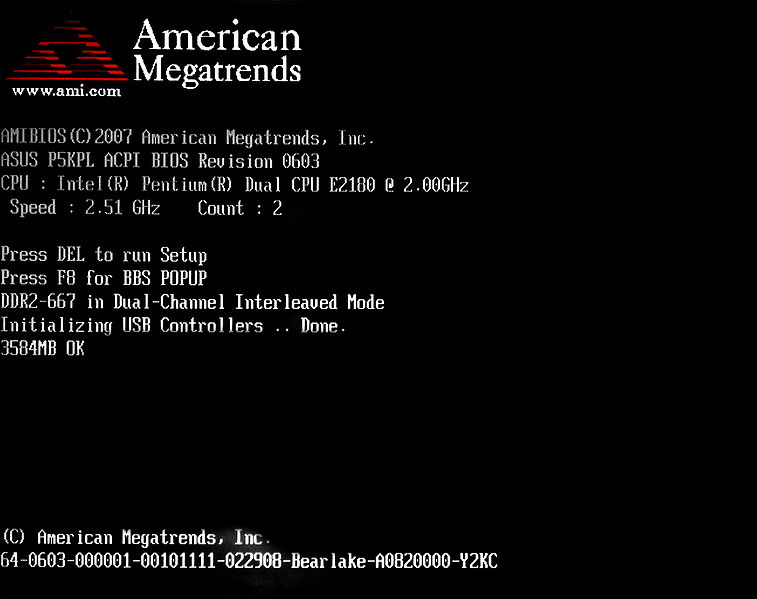
\includegraphics[scale=0.5,angle=-90]{pics/post.eps} \\
\end{center}
\vspace*{\fill}

\subsection{Typical Boot Sequence}
\vspace*{\fill}
\begin{center}
	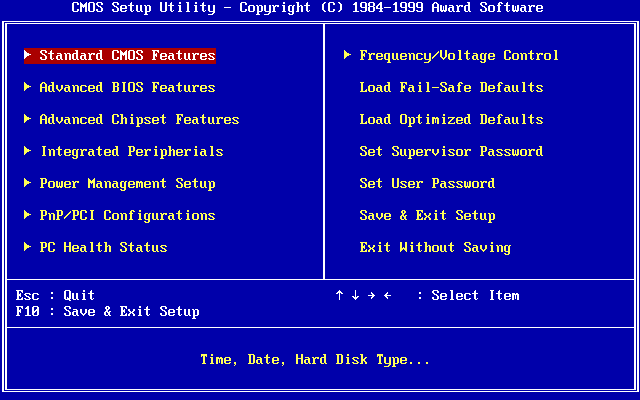
\includegraphics[scale=0.75,angle=-90]{pics/bios.eps} \\
\end{center}
\vspace*{\fill}

\subsection{Typical Boot Sequence}
\vspace*{\fill}
\begin{center}
	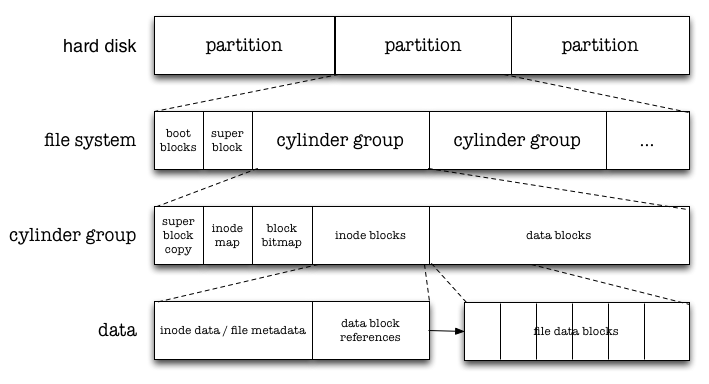
\includegraphics[scale=0.8,angle=-90]{pics/ufs-details.eps} \\
\end{center}
\vspace*{\fill}

\subsection{Typical Boot Sequence: BIOS and MBR}
\begin{minipage}[c]{0.7\textwidth}
\begin{itemize}
	\item first sector (512 bytes) of data storage device
	\item last two bytes contain signature \verb+0x55 0xAA+
	\item 64 bytes allocated for partition table (four possible
		partitions at 16 bytes each)
	\item 446 bytes for primary boot loader code
\end{itemize}
\end{minipage}
\begin{minipage}[c]{0.1\textwidth}
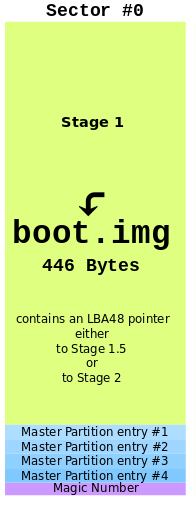
\includegraphics[scale=0.7]{pics/stage1.eps} \\
\end{minipage}


\subsection{Typical Boot Sequence}
\vspace*{\fill}
\begin{center}
	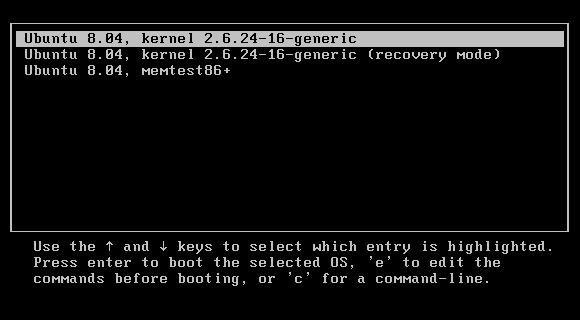
\includegraphics[scale=0.8,angle=-90]{pics/grub.eps} \\
\end{center}
\vspace*{\fill}


\subsection{Typical Boot Sequence}
\begin{itemize}
	\item {\bf P}ower-{\bf o}n {\bf S}elf-{\bf T}est
	\item primary boot loader (e.g. BIOS, UEFI, Open Firmware / OpenBoot)
	\item transfer of execution to {\bf M}aster {\bf B}oot {\bf R}ecord or perform netbooting
	\item Second-stage boot loader (e.g. GRUB)
	\item load kernel
	\item kernel transfers control to {\tt init(8)}
\end{itemize}

\subsection{Typical Boot Sequence}
\vspace*{\fill}
\begin{verbatim}
$ aws ec2 run-instances --image-id ami-3b361952
[wait... wait... wait...]
$ aws ec2 get-console-output --instance-id i-2fdb4701 | more
\end{verbatim}
\vspace*{\fill}


\subsection{Types of Software}

\subsection{Firmware}
\begin{center}
	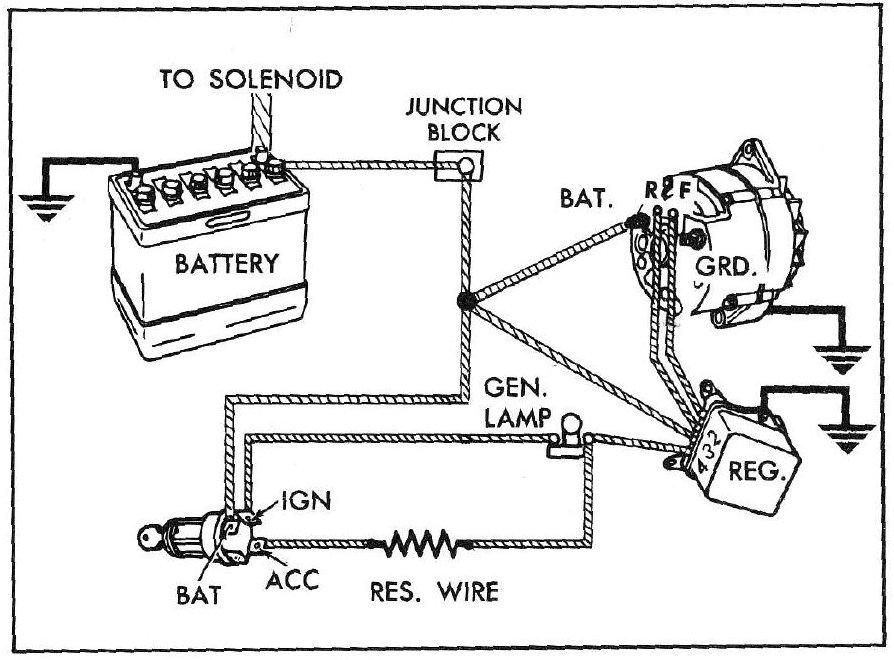
\includegraphics[scale=0.6,angle=-90]{pics/ignition-firmware.eps}
\end{center}

\subsection{Firmware}
\begin{center}
	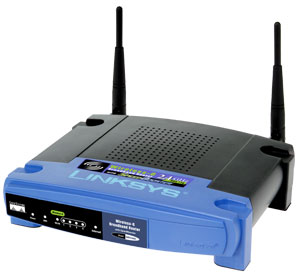
\includegraphics[scale=0.5,angle=-90]{pics/linksys.eps}
	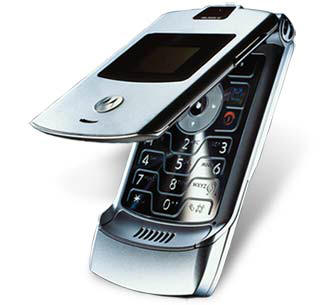
\includegraphics[scale=0.5,angle=-90]{pics/cell-phone.eps}
	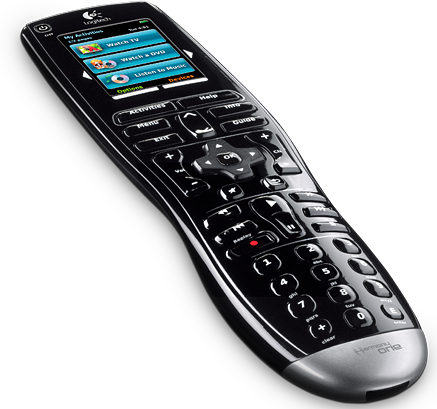
\includegraphics[scale=0.3,angle=-90]{pics/remote.eps}
\end{center}

\subsection{Firmware}
\begin{center}
	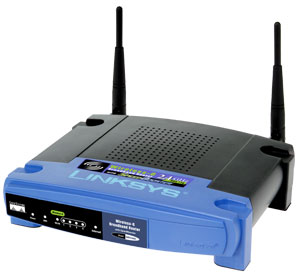
\includegraphics[scale=0.5,angle=-90]{pics/linksys.eps}
	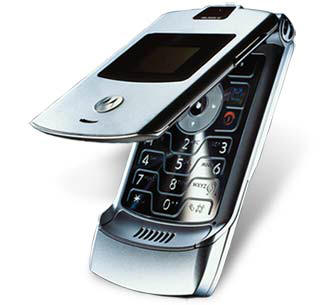
\includegraphics[scale=0.5,angle=-90]{pics/cell-phone.eps}
	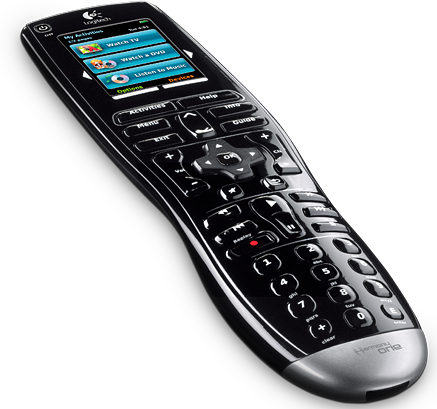
\includegraphics[scale=0.3,angle=-90]{pics/remote.eps} \\
	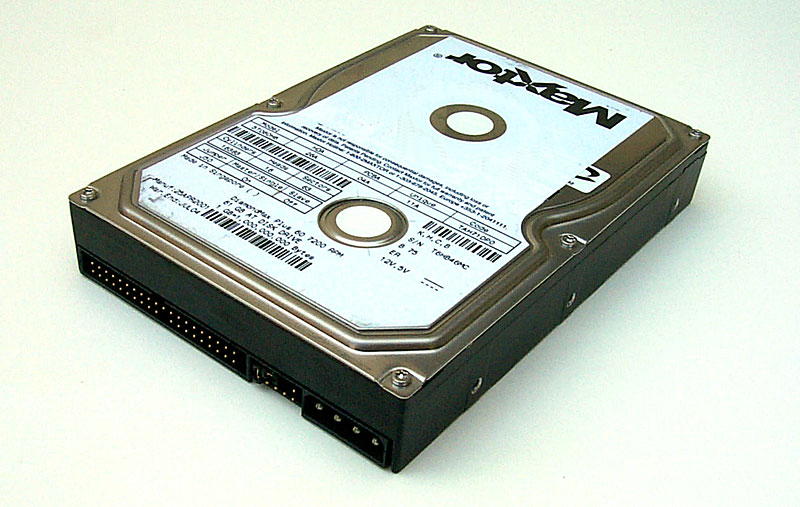
\includegraphics[scale=0.3,angle=-90]{pics/ide-drive.eps}
\end{center}



\subsection{Firmware}
\begin{center}
	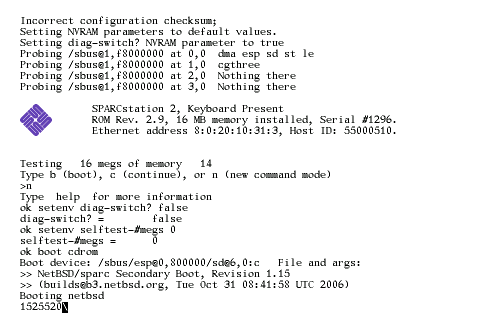
\includegraphics[scale=0.9,angle=-90]{pics/sun-firmware.eps}
\end{center}

\subsection{Firmware}
\begin{center}
	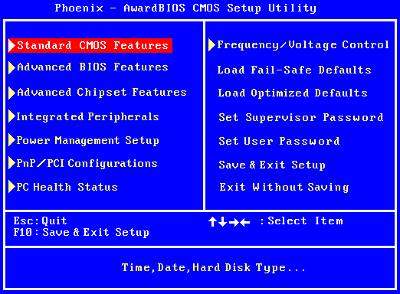
\includegraphics[scale=0.9,angle=-90]{pics/BIOS.eps}
\end{center}

\subsection{...}
\begin{center}
	
\includegraphics[scale=0.9]{pics/kfc1.eps}
\end{center}

\subsection{Kernel}
\begin{center}
        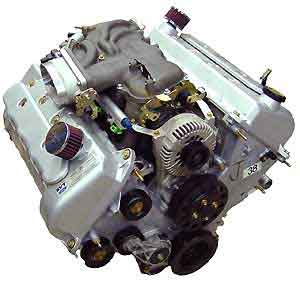
\includegraphics[scale=0.95,angle=-90]{pics/engine-kernel.eps}
\end{center}

\subsection{Kernel}
\small
\begin{verbatim}
Copyright (c) 1996, 1997, 1998, 1999, 2000, 2001, 2002, 2003, 2004, 2005,
    2006, 2007, 2008, 2009, 2010, 2011, 2012
    The NetBSD Foundation, Inc.  All rights reserved.

Copyright (c) 1982, 1986, 1989, 1991, 1993
    The Regents of the University of California.  All rights reserved.

NetBSD 6.1.2 (XEN3PAE_DOMU)
total memory = 615 MB
avail memory = 597 MB
mainbus0 (root)
hypervisor0 at mainbus0: Xen version 3.4.3.amazon
vcpu0 at hypervisor0: Intel(R) Xeon(R) CPU E5-2650 0 @ 2.00GHz, id 0x206d7
xenbus0 at hypervisor0: Xen Virtual Bus Interface
xencons0 at hypervisor0: Xen Virtual Console Driver
npx0 at hypervisor0: using exception 16
xbd0 at xenbus0 id 2049: Xen Virtual Block Device Interface
xbd1 at xenbus0 id 2050: Xen Virtual Block Device Interface
xennet0 at xenbus0 id 0: Xen Virtual Network Interface
xennet0: MAC address 22:00:0a:47:89:0e
balloon0 at xenbus0 id 0: Xen Balloon driver
balloon0: current reservation: 629760 KiB
xennet0: using RX copy mode
balloon0: current reservation: 157440 pages => target: 157440 pages
boot device: xbd1
root on xbd1a dumps on xbd1b
root file system type: ffs
Sat Feb  1 21:46:17 UTC 2014
\end{verbatim}
\Normalsize

\subsection{OS}
\begin{center}
	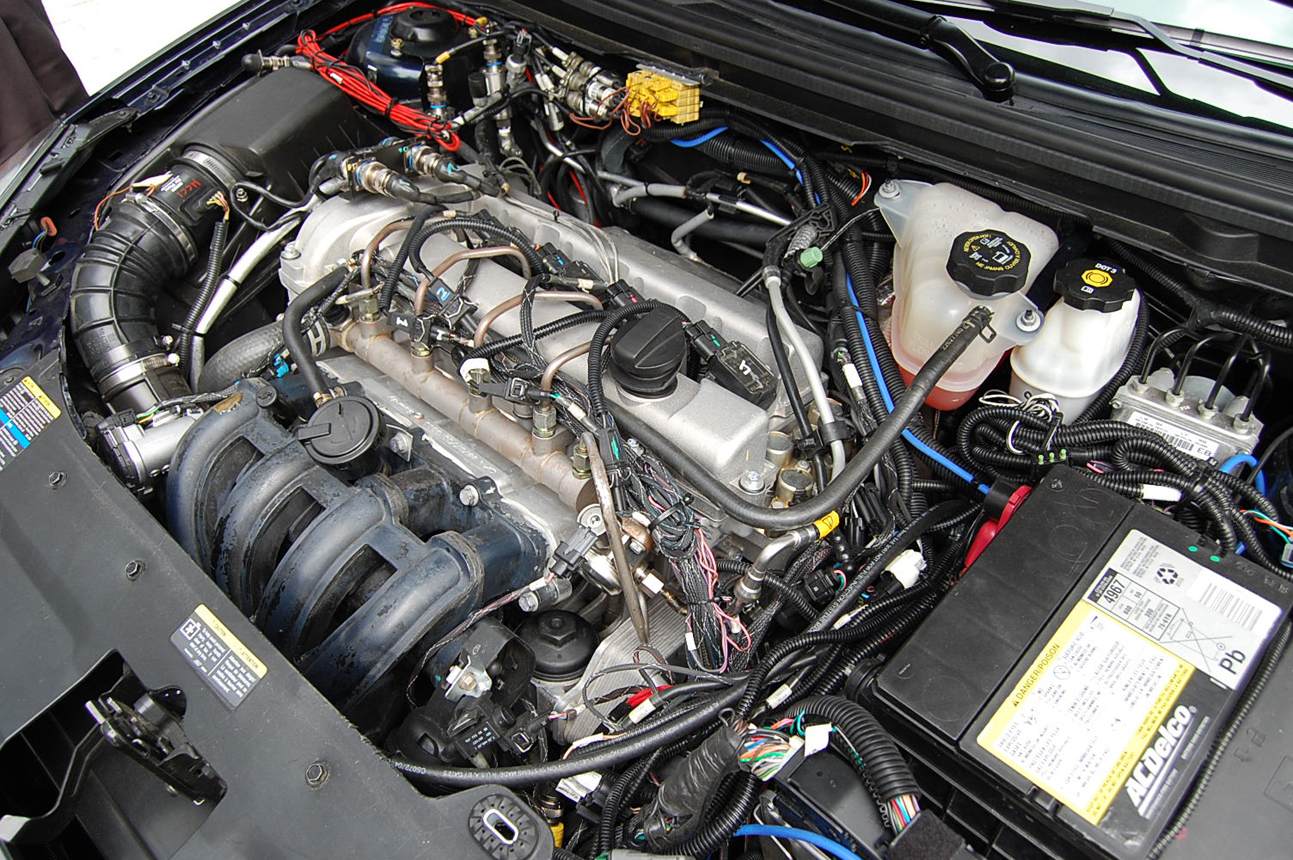
\includegraphics[scale=0.7,angle=-90]{pics/engine-os.eps}
\end{center}

\subsection{OS}
\begin{center}
	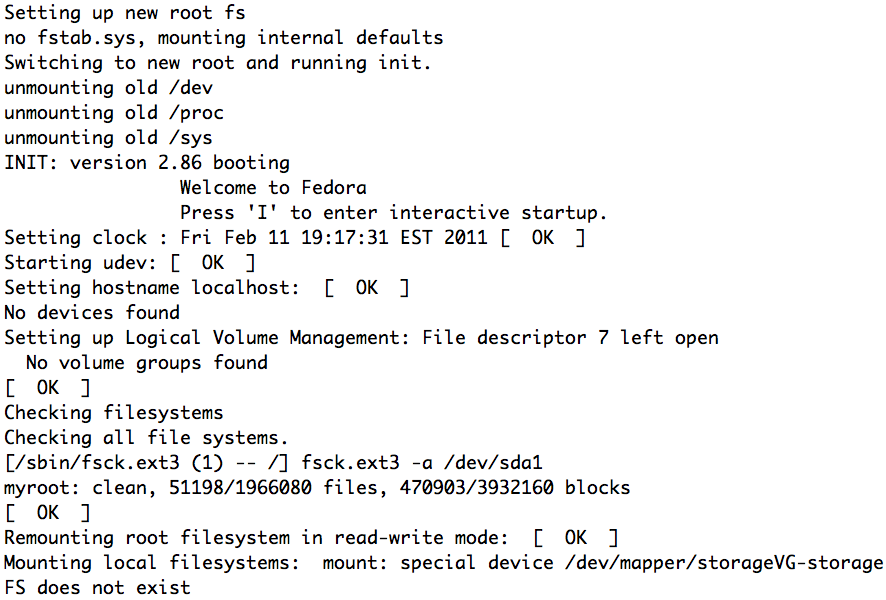
\includegraphics[scale=0.6,angle=-90]{pics/os-screenshot.eps}
\end{center}

\subsection{System Software}
\begin{center}
	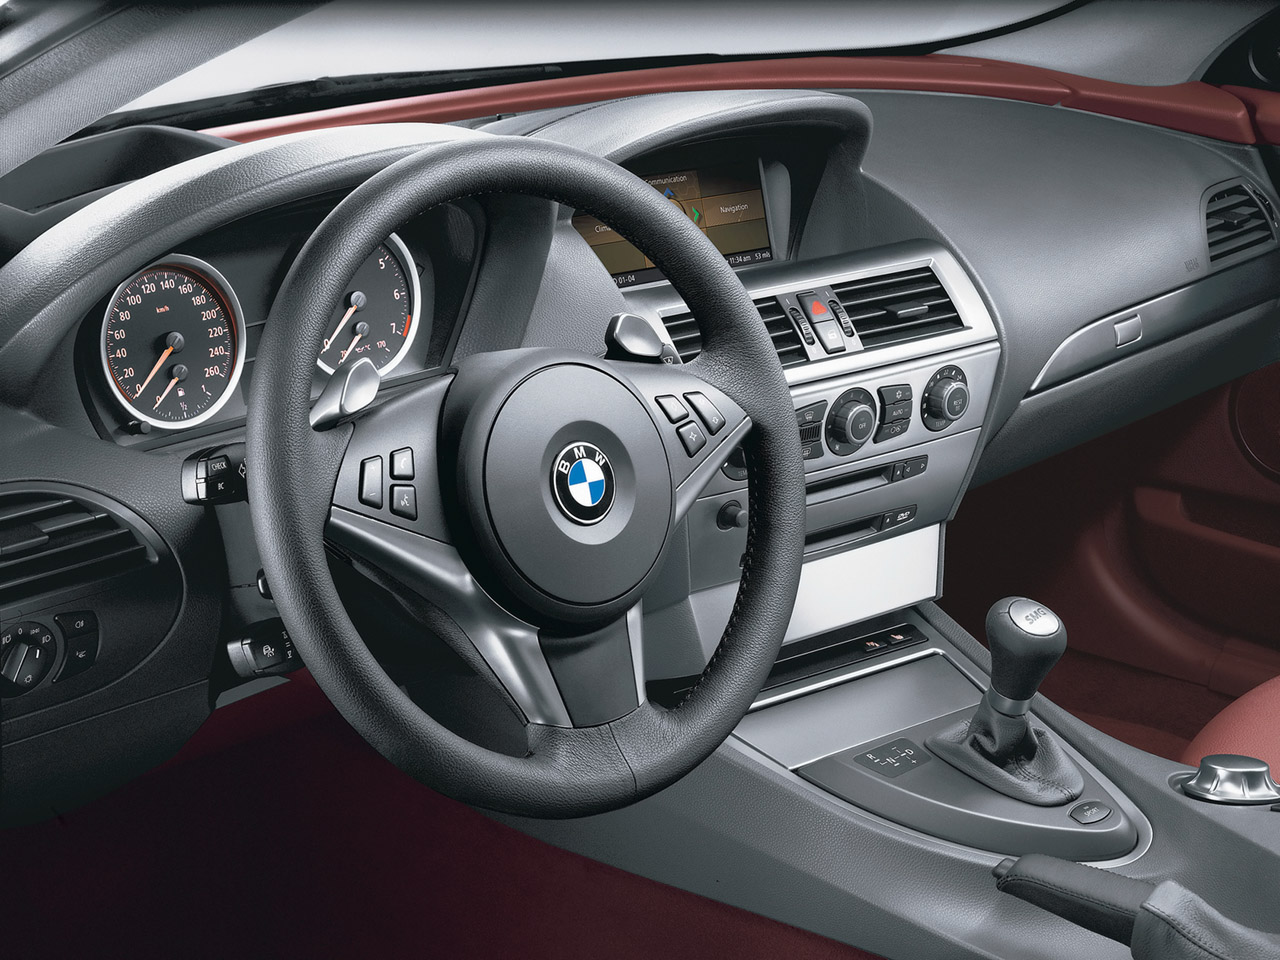
\includegraphics[scale=0.6,angle=-90]{pics/dashboard-system-software.eps}
\end{center}

\subsection{System Software}
\begin{center}
	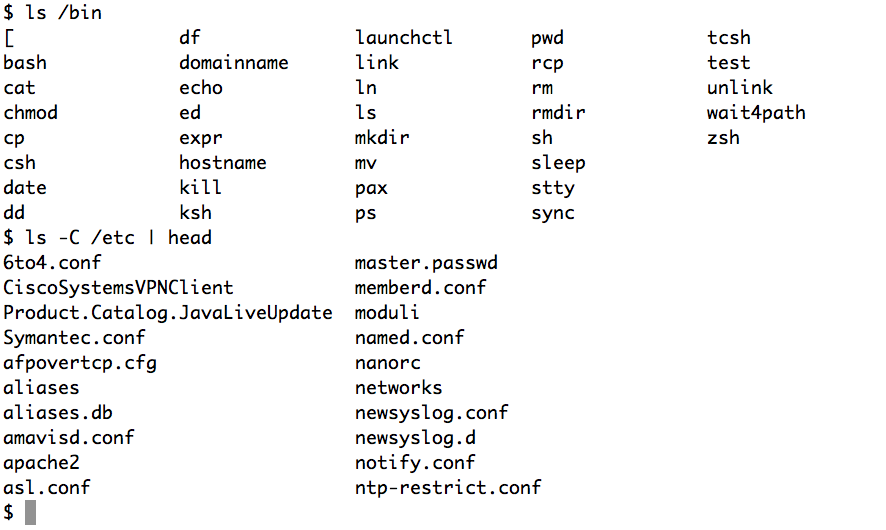
\includegraphics[scale=0.7,angle=-90]{pics/system-software.eps}
\end{center}

\subsection{Applications}
\begin{center}
	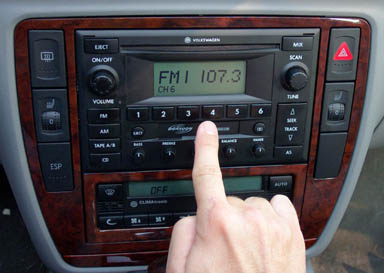
\includegraphics[scale=0.9,angle=-90]{pics/car_radio-applications.eps}
\end{center}

\subsection{Applications}
\begin{center}
	
\includegraphics[scale=0.3,angle=-90]{pics/python.eps}
	
\includegraphics[scale=0.3,angle=-90]{pics/logo_oracle.eps}
	\includegraphics[scale=0.8,angle=-90]{pics/apache.eps} \\
	
\includegraphics[scale=0.3,angle=-90]{pics/mysql.eps}
	
\includegraphics[scale=0.3,angle=-90]{pics/php-logo.eps}
\end{center}

\subsection{Types of Software}
\vfill
\begin{center}
	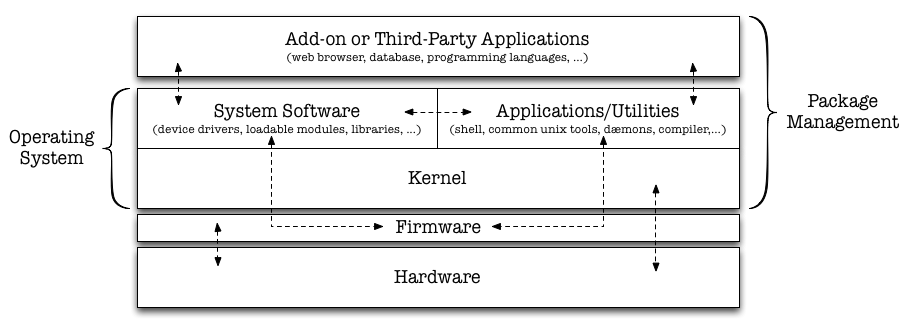
\includegraphics[scale=0.8,angle=-90]{pics/types-of-software.eps}
\end{center}
\vfill

\subsection{File System Hierarchy}
Layout of filesystem {\em should} be standardized.  Some UNIX versions adhere
to these standards, some are strongly influenced by tradition.
\\

{\tt man hier}

\subsection{File System Hierarchy}
\small
\begin{verbatim}
                     /          root directory of the system

                     /bin/      utilities used in both single and multi-user environments

                     /dev/      block, character and other special device files

                     /etc/      system configuration files and scripts

                     /lib/      dynamic linked libraries used by dynamic linked programs (such
                                as those in /bin/ and /sbin/) that cannot rely upon /usr/lib/
                                being available.

                     /sbin/     system programs and administration utilities used in both sin-
                                gle-user and multi-user environments

                     /tmp/      temporary files, usually a mfs(8) memory-based filesystem (the
                                contents of /tmp are usually not preserved across a system
                                reboot)

                     /usr/      contains the majority of the system utilities and files


                                bin/      common utilities, programming tools, and applica-
                                          tions

                                lib/      archive, profiled, position independent archive, and
                                          shared libraries

                                sbin/     system daemons and system utilities (normally exe-
                                          cuted by the super-user)

                                share/    architecture-independent text files
\end{verbatim}
\Normalsize

\newpage
\vspace*{\fill}
\begin{center}
	\Hugesize
		Software Installation Concepts \\ [1em]
	\hspace*{5mm}
	\blueline\\
	\hspace*{5mm}\\
		Operating System Installation
\end{center}
\vspace*{\fill}


\subsection{OS Installation}
\begin{center}
	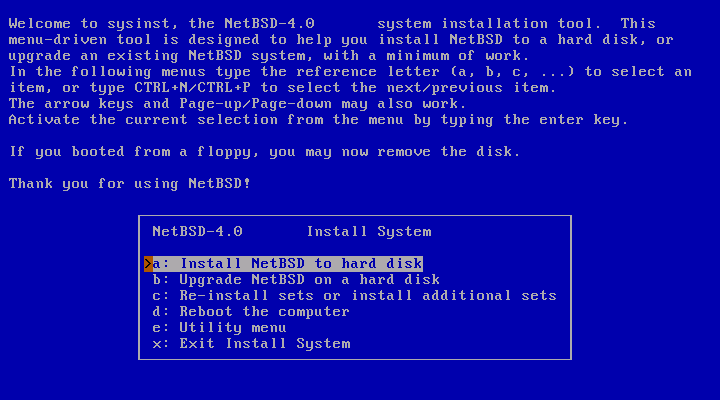
\includegraphics[scale=0.7,angle=-90]{pics/netbsd-install.eps}
\end{center}

\subsection{OS Installation}
Before installing, consider
\begin{itemize}
	\item purpose of machine
		\begin{itemize}
			\item choice of hardware
			\item disk partitioning scheme
			\item choice of filesystem
			\item which software to install
		\end{itemize}
	\item installation media
		\begin{itemize}
			\item network installation
			\item installation CD-ROMs
			\item customized boot media
		\end{itemize}
\end{itemize}

%\subsection{OS Installation}
%\vspace*{\fill}
%\begin{center}
%	\includegraphics[scale=0.8,angle=-90]{pics/inst-disklabel-partitions.eps}
%\end{center}
%\vspace*{\fill}
%
%\subsection{OS Installation}
%\vspace*{\fill}
%\begin{center}
%	\includegraphics[scale=0.55]{pics/disk.setup.eps}
%\end{center}
%\vspace*{\fill}
%
%\subsection{OS Installation}
%\vspace*{\fill}
%\begin{center}
%	\includegraphics[scale=0.8]{pics/install-ftp.eps}
%\end{center}
%\vspace*{\fill}
%
%\subsection{OS Installation}
%\vspace*{\fill}
%\begin{center}
%	\includegraphics[scale=0.8]{pics/nfssetup.eps}
%\end{center}
%\vspace*{\fill}
%

\subsection{OS Installation}
High-level overview:
\begin{itemize}
	\item hardware identification, provisioning, and registration
	\item base OS installation
	\item installation of add-on applications
	\item initial minimum system configuration [*]
	\item system registration
	\item system restart
\end{itemize}
\vspace*{\fill}
[*] system {\em deployment} $\cap$ system {\em configuration} \\
$ => $ configuration management

\subsection{Base OS Installation}
General steps:
\begin{itemize}
	\item boot from boot media (CD, network, ...)
	\item identify root device
	\item optionally identify additional devices
	\item create partition table / disklabel
	\item create filesystem(s)
	\item install MBR, bootblocks etc.
	\item install / copy / extract OS
	\item optionally add application software
	\item perform basic system configuration
	\item reboot
\end{itemize}

\subsection{OS Installation}
\small
\begin{verbatim}
# fdisk -f -u 0 -s 169/63/4194241 /dev/rwd0d
# fdisk -f -c /usr/mdec/mbr /dev/rwd0d
# fdisk -f -a -0 /dev/rwd0d
# disklabel -e -I wd0
[...]
4 partitions:
#      size   offset fstype [fsize bsize cpg/sgs]
a:  4194241       63 4.2BSD    0     0      0 # (Cyl.      0*- 4161*)
c:  4194241       63 4.2BSD    0     0      0 # (Cyl.      0*- 4161*)
d:  4194304        0 unused    0     0      0 # (Cyl.      0 - 4161*)
# /sbin/newfs -O 2 /dev/rwd0a
/dev/rwd0a: 2048.0MB (4194240 sectors) block size 16384,
        fragment size 2048 using 12 cylinder groups of
        170.67MB, 10923 blks, 21504 inodes.
super-block backups (for fsck_ffs -b #) at:
32, 349568, 699104, 1048640, 1398176, 1747712, 2097248, 2446784,
....................................................................
# mount -o async /dev/wd0a /mnt
# for pkg in base comp etc games man misc modules text kern-GENERIC; do
tar zxpf /i386/binary/sets/${pkg}.tgz -C /mnt
done
# cp /mnt/usr/mdec/boot /mnt/boot
# /usr/sbin/installboot -v -o timeout=5 /dev/rwd0a \
        /mnt/usr/mdec/bootxx_ffsv2
File system:       /dev/rwd0a
Primary bootstrap: /usr/mdec/bootxx_ffsv2
Boot options:      timeout 5, flags 0, speed 9600, ioaddr 0, console pc
# cd /mnt/dev && ./MAKEDEV all
# shutdown -r now
\end{verbatim}
\Normalsize

\subsection{Post Installation}
\vspace*{\fill}
\begin{center}
	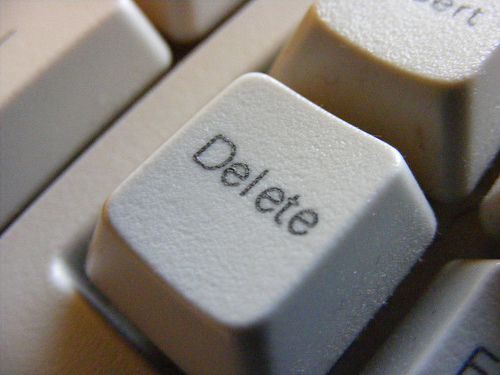
\includegraphics[scale=0.8,angle=-90]{pics/delete.eps}
\end{center}
\vspace*{\fill}

\subsection{Post Installation}
\vspace*{\fill}
\begin{center}
	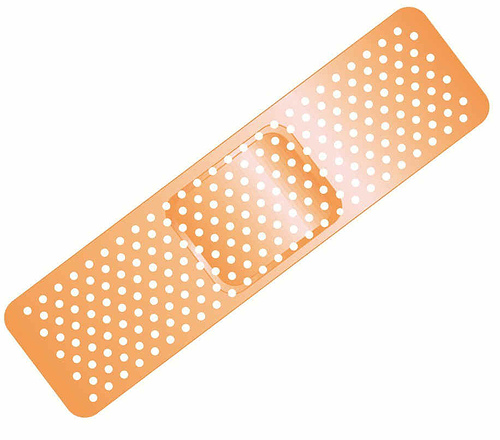
\includegraphics[scale=0.7]{pics/bandaid.eps}
\end{center}
\vspace*{\fill}

\subsection{Post Installation}
\vspace*{\fill}
\begin{center}
	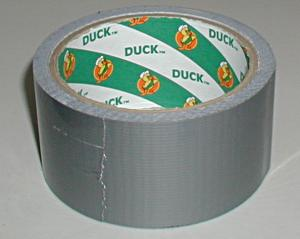
\includegraphics[scale=1.0,angle=-90]{pics/duck_tape.eps}
\end{center}
\vspace*{\fill}

\newpage
\vspace*{\fill}
\begin{center}
    \Hugesize
        Hooray! \\ [1em]
    \hspace*{5mm}
    \blueline\\
    \hspace*{5mm}\\
        5 Minute Break
\end{center}
\vspace*{\fill}

\newpage
\vspace*{\fill}
\begin{center}
	\Hugesize
		Software Installation Concepts \\ [1em]
	\hspace*{5mm}
	\blueline\\
	\hspace*{5mm}\\
		System Software vs. Third Party Software
\end{center}
\vspace*{\fill}

\subsection{What's what?}
\begin{center}
	\includegraphics[scale=0.7]{pics/os.eps}
\end{center}

\subsection{What's what?}
\begin{center}
	
\includegraphics[scale=0.3,angle=-90]{pics/python.eps}
	
\includegraphics[scale=0.3,angle=-90]{pics/logo_oracle.eps}
	\includegraphics[scale=0.8,angle=-90]{pics/apache.eps} \\
	
\includegraphics[scale=0.3,angle=-90]{pics/mysql.eps}
	
\includegraphics[scale=0.3,angle=-90]{pics/php-logo.eps}
\end{center}

\subsection{What's what?}
\begin{center}
	
\includegraphics[scale=0.9]{pics/leftshark.eps} \\
Superfish
\end{center}

\subsection{Types of Software}
\vfill
\begin{center}
	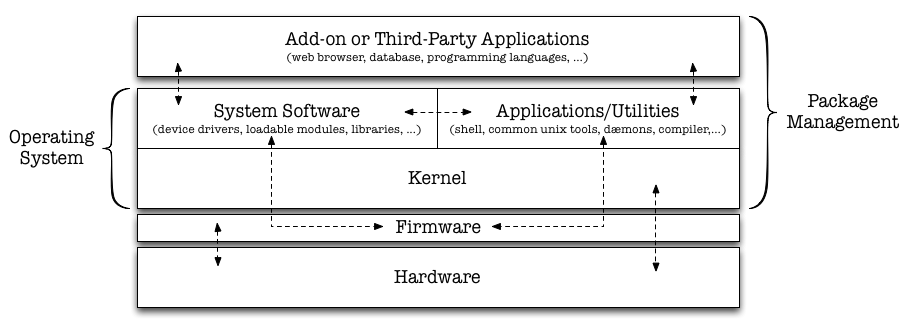
\includegraphics[scale=0.8,angle=-90]{pics/types-of-software.eps}
\end{center}
\vfill




\subsection{System Software vs. Third Party Software}
Consider:
\begin{itemize}
	\item OS upgrades vs. software upgrades
\end{itemize}

\subsection{System Software vs. Third Party Software}
Consider:
\begin{itemize}
	\item OS upgrades vs. software upgrades
	\item location of configuration files
\end{itemize}

\subsection{System Software vs. Third Party Software}
Consider:
\begin{itemize}
	\item OS upgrades vs. software upgrades
	\item location of configuration files
	\item duplicates or conflicting versions in the base system vs. the
		add-ons
\end{itemize}

\subsection{System Software vs. Third Party Software}
Consider:
\begin{itemize}
	\item OS upgrades vs. software upgrades
	\item location of configuration files
	\item duplicates or conflicting versions in the base system vs. the
		add-ons
	\item startup scripts, d{\ae}mons
\end{itemize}

\subsection{System Software vs. Third Party Software}
Consider:
\begin{itemize}
	\item OS upgrades vs. software upgrades
	\item location of configuration files
	\item duplicates or conflicting versions in the base system vs. the
		add-ons
	\item startup scripts, d{\ae}mons
	\item location of third party software
\end{itemize}

\subsection{System Software vs. Third Party Software}
Consider:
\begin{itemize}
	\item OS upgrades vs. software upgrades
	\item location of configuration files
	\item duplicates or conflicting versions in the base system vs. the
		add-ons
	\item startup scripts, d{\ae}mons
	\item location of third party software
	\item dependencies
\end{itemize}

\subsection{System Software vs. Third Party Software}
Consider:
\begin{itemize}
	\item OS upgrades vs. software upgrades
	\item location of configuration files
	\item duplicates or conflicting versions in the base system vs. the
		add-ons
	\item startup scripts, d{\ae}mons
	\item location of third party software
	\item dependencies
	\item installation by hand and/or installation using a package manager
\end{itemize}


\subsection{System Software vs. Third Party Software}
Consider:
\begin{itemize}
	\item OS upgrades vs. software upgrades
	\item location of configuration files
	\item duplicates or conflicting versions in the base system vs. the
		add-ons
	\item startup scripts, d{\ae}mons
	\item location of third party software
	\item dependencies
	\item installation by hand and/or installation using a package manager
	\item proprietary third party software
\end{itemize}


\newpage
\vspace*{\fill}
\begin{center}
	\Hugesize
		Software Installation Concepts \\ [1em]
	\hspace*{5mm}
	\blueline\\
	\hspace*{5mm}\\
		Practical Exercises
\end{center}
\vspace*{\fill}

\subsection{Package management basics}
\vfill
{\tt https://www.cs.stevens.edu/\~{}jschauma/615/pkg-exercise.html}
\vfill

\subsection{Binary vs. Source installation}
Benefits of binary installation:
\begin{itemize}
	\item packaged by "vendor" $\rightarrow$ support, ease of installation
	\item faster
	\item uses less space
	\item may be only possibility
	\item able to integrate into your full OS image build
	\item may be possible to deploy across large numbers of hosts
\end{itemize}

\subsection{Binary vs. Source installation}
Disadvantages of binary installation:
\begin{itemize}
	\item complex dependencies
	\item installation procedure may be cumbersome
	\item your OS may not be officially supported
	\item installation scripts may be busted
	\item limited control over where files are installed
	\item missing or not-needed features enabled
	\item you have to trust the package provider
\end{itemize}

\subsection{Binary vs. Source installation}
Benefits of source installation:
\begin{itemize}
	\item full control over
		\begin{itemize}
			\item installation location
			\item compiler flags, optimization, enabled features
			\item dependencies
		\end{itemize}
	\item make things work even if your OS is not officially supported
	\item ability to patch source (features, security etc.)
	\item able to integrate into your full OS image build
\end{itemize}

\subsection{Binary vs. Source installation}
Disadvantages of source installation:
\begin{itemize}
	\item complex dependencies
	\item may take time
	\item requires more detailed knowledge
	\item a lot of software is done poorly
	\item not all software is available in source form
	\item you have to trust the source code provider
\end{itemize}


\subsection{Why use a Package Management System?}
\begin{itemize}
	\item easy and scalable installation of software
	\item automatic resolution of software dependencies
	\item package and file inventory \\
\begin{verbatim}
linux-lab$ dpkg -l
[...]
linux-lab$ dpkg -L tcpdump
[...]
linux-lab$ dpkg-query -S /usr/lib/libsqlite.so.0.8.6 /usr/bin/sqlite3
[...]

\end{verbatim}
\end{itemize}

\subsection{Why use a Package Management System?}
\begin{itemize}
	\item easy and scalable installation of software
	\item automatic resolution of software dependencies
	\item package and file inventory
	\item integration into OS
	\item package and file integrity checks \\
\begin{verbatim}
$ rpm -Va
[...]
missing     /etc/pki/CA/private (Permission denied)
S.5.....  c /etc/pki/tls/certs/ca-bundle.crt
.......T  c /etc/libuser.conf
..?.....  c /etc/tcsd.conf
missing   c /etc/logrotate.d/syslog
[...]
\end{verbatim}
\end{itemize}

\subsection{Managing Security Patches and Software Upgrades}
How many known vulnerabilities (unique CVEs and affected packages) exist
in each of the Fedora and Ubuntu instances?

\begin{verbatim}
ubuntu$ sudo apt-get install debsecan
ubuntu$ debsecan
\end{verbatim}

\begin{verbatim}
fedora$ yum list-security
fedora$ yum info-security
\end{verbatim}

\subsection{Special Purpose Package Managers}
\vfill
\begin{center}
	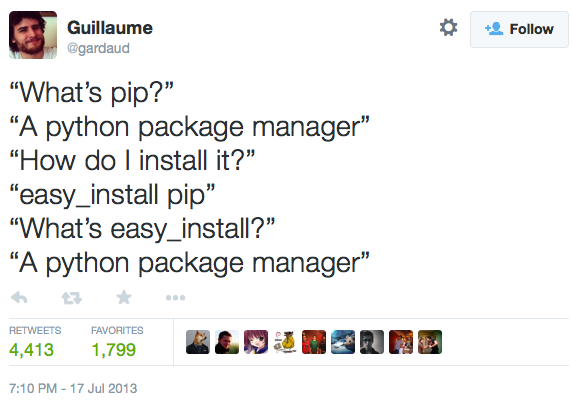
\includegraphics[scale=0.8,angle=-90]{pics/pip.eps}
\end{center}
\vfill

\subsection{Special Purpose Package Managers}
\vfill
\begin{center}
	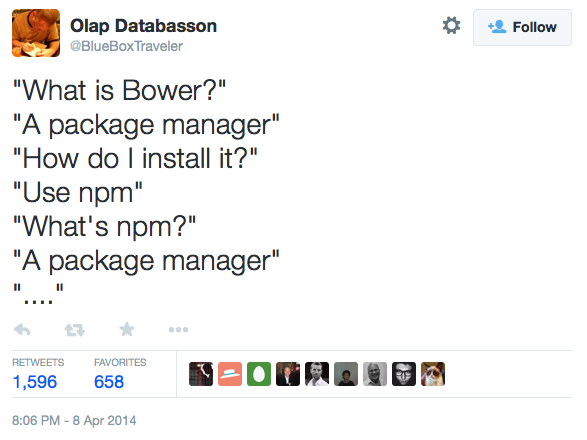
\includegraphics[scale=0.8,angle=-90]{pics/bower.eps}
\end{center}
\vfill


\subsection{Special Purpose Package Managers}
Most programming languages or environments come with their own "package
management" solutions, often integrating/mixing with a "build system".
\begin{itemize}
	\item Common Lisp $=>$ quicklisp
	\item NodeJS $=>$ npm
	\item Perl $=>$ CPAN
	\item Python $=>$ easy-install, pip, pants, setuptools, ...
	\item Ruby $=>$ gems, rvm, rake
	\item Scala $=>$ sbt
	\item YourFavoriteThing $=>$ ItsOwnGizmo
\end{itemize}

\subsection{You don't get to choose.}
\Huge
\vfill
\begin{center}
	You routinely have to build from source {\em and} (re-)package your software.
\end{center}
\vfill
\Normalsize

\subsection{HW \#2}

Create an RPM for 'awscli'.
\\

Detailed homework assignment posted at
\verb+https://www.cs.stevens.edu/~jschauma/615/s15-hw2.html+


\subsection{Links}
\begin{itemize}
	\item \verb+http://www.pathname.com/fhs/+
	\item hier(7)
	\item your package managers' manual pages
		\begin{itemize}
			\item pkg\_info(1)
			\item pkginfo(1), pkgadd(1M)
			\item rpm(1)
			\item ...
		\end{itemize}
	\item \verb+http://www.pkgsrc.org/+
\end{itemize}

\end{document}
